%%%%%%%%%%%%%%%%%%%%%%%%%%%%%%%%%%%%%%%%%%%%%%%%%%%%%%%%%%%%%%%%%%%%%%%%%%%%%%%%%%%%%%%%%%%%%%%%%%%%%%%%%%%%%%%%%%%%%%%%%%%%%%%%%%%%%%%%%%%%%%%%%%%%%%%%%%%%%%%%%%%
% Written By Michael Brodskiy
% Class: Electricity & Magnetism
% Professor: D. Wood
%%%%%%%%%%%%%%%%%%%%%%%%%%%%%%%%%%%%%%%%%%%%%%%%%%%%%%%%%%%%%%%%%%%%%%%%%%%%%%%%%%%%%%%%%%%%%%%%%%%%%%%%%%%%%%%%%%%%%%%%%%%%%%%%%%%%%%%%%%%%%%%%%%%%%%%%%%%%%%%%%%%

\include{Includes.tex}

\title{Homework 4}
\date{October 12, 2023}
\author{Michael Brodskiy\\ \small Professor: D. Wood}

\begin{document}

\maketitle

\begin{enumerate}

  \item Consider an infinite grounded conducting plane bent at a $90^{\circ}$ angle between the $yz$ and $xz$ planes as shown, with a charge placed at $x = 4a$, $y = a$. Use appropriate image charge(s) to find an expression for the potential $V(x,y,z)$ in the region $x > 0$, $y > 0$.

    First, we know that the image charges assume the following layout:

    \begin{figure}[H]
      \centering
      \tikzset{every picture/.style={line width=0.75pt}} %set default line width to 0.75pt        

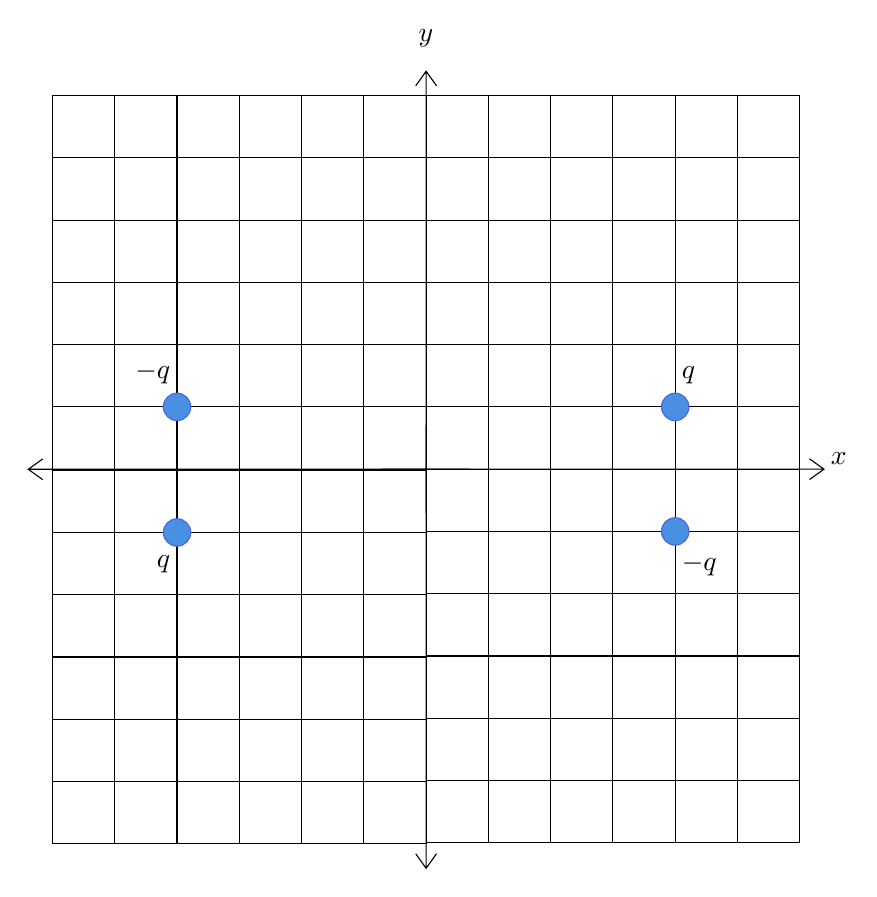
\begin{tikzpicture}[x=0.75pt,y=0.75pt,yscale=-1,xscale=1]
%uncomment if require: \path (0,657); %set diagram left start at 0, and has height of 657

%Shape: Axis 2D [id:dp1373512094917413] 
\draw  (259,275.7) -- (472,275.7)(280.3,84) -- (280.3,297) (465,270.7) -- (472,275.7) -- (465,280.7) (275.3,91) -- (280.3,84) -- (285.3,91)  ;
%Shape: Axis 2D [id:dp329188015017823] 
\draw  (301.6,275.76) -- (88.6,275.76)(280.3,468) -- (280.3,254.4) (95.6,280.76) -- (88.6,275.76) -- (95.6,270.76) (285.3,461) -- (280.3,468) -- (275.3,461)  ;
%Shape: Grid [id:dp7539739677566268] 
\draw  [draw opacity=0] (100.3,276.2) -- (280.3,276.2) -- (280.3,456.2) -- (100.3,456.2) -- cycle ; \draw   (130.3,276.2) -- (130.3,456.2)(160.3,276.2) -- (160.3,456.2)(190.3,276.2) -- (190.3,456.2)(220.3,276.2) -- (220.3,456.2)(250.3,276.2) -- (250.3,456.2) ; \draw   (100.3,306.2) -- (280.3,306.2)(100.3,336.2) -- (280.3,336.2)(100.3,366.2) -- (280.3,366.2)(100.3,396.2) -- (280.3,396.2)(100.3,426.2) -- (280.3,426.2) ; \draw   (100.3,276.2) -- (280.3,276.2) -- (280.3,456.2) -- (100.3,456.2) -- cycle ;
%Shape: Grid [id:dp2853097292529867] 
\draw  [draw opacity=0] (280.3,275.7) -- (460.3,275.7) -- (460.3,455.7) -- (280.3,455.7) -- cycle ; \draw   (310.3,275.7) -- (310.3,455.7)(340.3,275.7) -- (340.3,455.7)(370.3,275.7) -- (370.3,455.7)(400.3,275.7) -- (400.3,455.7)(430.3,275.7) -- (430.3,455.7) ; \draw   (280.3,305.7) -- (460.3,305.7)(280.3,335.7) -- (460.3,335.7)(280.3,365.7) -- (460.3,365.7)(280.3,395.7) -- (460.3,395.7)(280.3,425.7) -- (460.3,425.7) ; \draw   (280.3,275.7) -- (460.3,275.7) -- (460.3,455.7) -- (280.3,455.7) -- cycle ;
%Shape: Grid [id:dp3861257807049996] 
\draw  [draw opacity=0] (280.3,95.7) -- (460.3,95.7) -- (460.3,275.7) -- (280.3,275.7) -- cycle ; \draw   (310.3,95.7) -- (310.3,275.7)(340.3,95.7) -- (340.3,275.7)(370.3,95.7) -- (370.3,275.7)(400.3,95.7) -- (400.3,275.7)(430.3,95.7) -- (430.3,275.7) ; \draw   (280.3,125.7) -- (460.3,125.7)(280.3,155.7) -- (460.3,155.7)(280.3,185.7) -- (460.3,185.7)(280.3,215.7) -- (460.3,215.7)(280.3,245.7) -- (460.3,245.7) ; \draw   (280.3,95.7) -- (460.3,95.7) -- (460.3,275.7) -- (280.3,275.7) -- cycle ;
%Shape: Grid [id:dp2044452336417133] 
\draw  [draw opacity=0] (100.3,95.7) -- (280.3,95.7) -- (280.3,275.7) -- (100.3,275.7) -- cycle ; \draw   (130.3,95.7) -- (130.3,275.7)(160.3,95.7) -- (160.3,275.7)(190.3,95.7) -- (190.3,275.7)(220.3,95.7) -- (220.3,275.7)(250.3,95.7) -- (250.3,275.7) ; \draw   (100.3,125.7) -- (280.3,125.7)(100.3,155.7) -- (280.3,155.7)(100.3,185.7) -- (280.3,185.7)(100.3,215.7) -- (280.3,215.7)(100.3,245.7) -- (280.3,245.7) ; \draw   (100.3,95.7) -- (280.3,95.7) -- (280.3,275.7) -- (100.3,275.7) -- cycle ;
%Shape: Circle [id:dp6814120704702491] 
\draw  [color={rgb, 255:red, 74; green, 99; blue, 226 }  ,draw opacity=1 ][fill={rgb, 255:red, 74; green, 144; blue, 226 }  ,fill opacity=1 ] (393.7,245.7) .. controls (393.7,242.05) and (396.65,239.1) .. (400.3,239.1) .. controls (403.95,239.1) and (406.9,242.05) .. (406.9,245.7) .. controls (406.9,249.35) and (403.95,252.3) .. (400.3,252.3) .. controls (396.65,252.3) and (393.7,249.35) .. (393.7,245.7) -- cycle ;
%Shape: Circle [id:dp37300952646152163] 
\draw  [color={rgb, 255:red, 74; green, 99; blue, 226 }  ,draw opacity=1 ][fill={rgb, 255:red, 74; green, 144; blue, 226 }  ,fill opacity=1 ] (393.7,305.7) .. controls (393.7,302.05) and (396.65,299.1) .. (400.3,299.1) .. controls (403.95,299.1) and (406.9,302.05) .. (406.9,305.7) .. controls (406.9,309.35) and (403.95,312.3) .. (400.3,312.3) .. controls (396.65,312.3) and (393.7,309.35) .. (393.7,305.7) -- cycle ;
%Shape: Circle [id:dp5860262256290361] 
\draw  [color={rgb, 255:red, 74; green, 99; blue, 226 }  ,draw opacity=1 ][fill={rgb, 255:red, 74; green, 144; blue, 226 }  ,fill opacity=1 ] (153.7,306.2) .. controls (153.7,302.55) and (156.65,299.6) .. (160.3,299.6) .. controls (163.95,299.6) and (166.9,302.55) .. (166.9,306.2) .. controls (166.9,309.85) and (163.95,312.8) .. (160.3,312.8) .. controls (156.65,312.8) and (153.7,309.85) .. (153.7,306.2) -- cycle ;
%Shape: Circle [id:dp11907902437511675] 
\draw  [color={rgb, 255:red, 74; green, 99; blue, 226 }  ,draw opacity=1 ][fill={rgb, 255:red, 74; green, 144; blue, 226 }  ,fill opacity=1 ] (153.7,245.7) .. controls (153.7,242.05) and (156.65,239.1) .. (160.3,239.1) .. controls (163.95,239.1) and (166.9,242.05) .. (166.9,245.7) .. controls (166.9,249.35) and (163.95,252.3) .. (160.3,252.3) .. controls (156.65,252.3) and (153.7,249.35) .. (153.7,245.7) -- cycle ;

% Text Node
\draw (474,266.4) node [anchor=north west][inner sep=0.75pt]    {$x$};
% Text Node
\draw (280.22,73.6) node [anchor=south] [inner sep=0.75pt]    {$y$};
% Text Node
\draw (402.3,235.7) node [anchor=south west] [inner sep=0.75pt]    {$q$};
% Text Node
\draw (402.3,315.7) node [anchor=north west][inner sep=0.75pt]    {$-q$};
% Text Node
\draw (158.3,316.2) node [anchor=north east] [inner sep=0.75pt]    {$q$};
% Text Node
\draw (158.3,235.7) node [anchor=south east] [inner sep=0.75pt]    {$-q$};


\end{tikzpicture}

      \caption{The Layout of Image Charges}
      \label{fig:1}
    \end{figure}

    By the principle of superposition, we know that the voltage at a point will simply be the sum of all voltages. Thus, we can assign each charge, starting with the top left, a distance $d_1-d_4$. We can find the following:

    $$d_1=\sqrt{(x+4a)^2+(y-a)^2+z^2}=\sqrt{x^2+y^2+z^2+17a^2+8ax-2ay}$$
    $$d_2=\sqrt{(x-4a)^2+(y-a)^2+z^2}=\sqrt{x^2+y^2+z^2+17a^2-8ax-2ay}$$
    $$d_3=\sqrt{(x+4a)^2+(y+a)^2+z^2}=\sqrt{x^2+y^2+z^2+17a^2+8ax+2ay}$$
    $$d_4=\sqrt{(x-4a)^2+(y+a)^2+z^2}=\sqrt{x^2+y^2+z^2+17a^2-8ax+2ay}$$

    We can then write the voltage as:

    $$V=V_1+V_2+V_3+V_4$$
    $$=\frac{q}{4\pi\varepsilon_o}\left[  -\frac{1}{d_1}+\frac{1}{d_2}+\frac{1}{d_3}-\frac{1}{d_4}\right]$$

    This gives us the final expression:

    $$V(x,y,z)=\frac{q}{4\pi\varepsilon_o}\left[ \frac{1}{\sqrt{(x-4a)^2+(y-a)^2+z^2}}+\frac{1}{\sqrt{(x+4a)^2+(y+a)^2+z^2}}$$
    $$\left -\frac{1}{\sqrt{(x+4a)^2+(y-a)^2+z^2}}-\frac{1}{\sqrt{(x-4a)^2+(y+a)^2+z^2}} \right]$$

  \item The boundary at $x = 0$ consists of two metal strips: one, from $y = 0$ to $y = a/2$ is held at a constant potential $+V_0$ and the other, from $y = a/2$ to $y = a$ is held at a constant potential of $−V_0$ . Solve for the potential $V(x,y,z)$ inside the slot. Feel free to use the relevant results from Example 3.3 or from lecture as a starting point.

    We can first write the Laplace equation:

    $$\frac{\partial^2V}{\partial x^2}+\frac{\partial^2V}{\partial y^2}=0$$

    Given the boundary conditions, we may write:

    $$V(x,y)=\sum_{n=1}^\infty c_ne^{-\frac{n\pi x}{a}}\sin\left( \frac{n\pi y}{a} \right)$$

    We find the value of $c_n$ by rearranging:

    $$c_n=\frac{2}{a}\left[\int_0^{\frac{a}{2}}V_o\sin\left( \frac{n\pi y}{a} \right)\,dy-\int_{\frac{a}{2}}^{a}V_o\sin\left( \frac{n\pi y}{a} \right)\,dy\right]$$
    $$c_n=\frac{2V_oa}{an\pi}\left[\left( -\cos\left( \frac{n\pi y}{a} \right)\Big|_0^{\frac{a}{2}} \right)+\left( \cos\left( \frac{n\pi y}{a} \right)\Big|_{\frac{a}{2}}^{a} \right)\right]$$
    $$c_n=\frac{2V_o}{n\pi}\left[1+\cos(n\pi)-2\cos\left( \frac{n\pi}{2} \right)\right]$$

    From this, we can see that $c_n=0$ for any odd values of $n$. Furthermore, if $n$ is a multiple of $4$, $c_n=0$ as well. Thus, we can see that $c_n$ is non-zero only for $n=2,6,10,\ldots$ for which:

    $$c_n=\frac{8V_o}{n\pi}$$

    We can now substitute into our previous equation to obtain:

    $$\boxed{V(x,y)=\frac{8V_o}{\pi}\sum_{n=2,6,10,\ldots}^\infty\frac{e^{-\frac{n\pi x}{a}\sin\left( \frac{n\pi y}{a} \right)}}{n}}$$

  \item Consider a long (semi-infinite) rectangular conducting pipe oriented $V_0$ parallel to the $z$-axis, with dimensions $a\times b$ in the $xy$-plane. The pipe itself is grounded, and the rectangle at the closed end is at a constant potential $V_0$ . Find an expression for the potential everywhere inside the pipe (for $z > 0$).

    For this problem, we must apply a three dimensional Laplace equation, with boundary conditions:

    $$\frac{\partial^2 V}{\partial x^2}+\frac{\partial^2V}{\partial y^2}+\frac{\partial^2V}{\partial z^2}=0\Rightarrow \left\{\begin{array}{c c}V=0, & \left[\begin{array}{c} x=0\\x=a\\y=0\\y=b\end{array}\\V=V_o, & z=0\\V\to0, & z\to\infty\end{array}$$

        We can then divide the equation by $V(x,y,z)$ to obtain:

        $$\underbrace{\frac{1}{V_x}\frac{\partial^2V_x}{\partial x^2}}_{-A^2}+\underbrace{\frac{1}{V_y}\frac{\partial^2V_y}{\partial y^2}}_{-B^2}+\underbrace{\frac{1}{V_z}\frac{\partial^2V_z}{\partial z^2}}_{C^2}=0$$

        Note: the $z^2$ term will be positive to guarantee at least one exponentially decaying solution. This gives us:

        $$C^2=A^2+B^2$$
        $$\frac{\partial^2V_x}{\partial x^2}=-A^2V_x\quad\quad\frac{\partial^2V_y}{\partial y^2}=-B^2V_y\quad\quad\frac{\partial^2V_z}{\partial z^2}=(A^2+B^2)V_z$$

        Given this form, we know the solutions will be of form:

        $$V_x=P\sin(Ax)+Q\cos(Ax)$$
        $$V_y=R\sin(Bx)+S\cos(Bx)$$
        $$V_z=Te^{\sqrt{A^2+B^2}z}+Ue^{-\sqrt{A^2+B^2}z}$$

        To simplify, we can now apply some of our boundary conditions from above. Let us first apply the last condition ($V_z\to0$ as $z\to\infty$). This gives us $S=0$:

        $$V_x=P\sin(Ax)+Q\cos(Ax)$$
        $$V_y=R\sin(Bx)+S\cos(Bx)$$
        $$V_z=Ue^{-\sqrt{A^2+B^2}z}$$

        Now, by conditions one and three, we know that, when $V=0$, $x=0$ and $y=0$, giving $Q=0$ and $T=0$:

        $$V_x=P\sin(Ax)$$
        $$V_y=R\sin(Bx)$$
        $$V_z=Ue^{-\sqrt{A^2+B^2}z}$$

        From conditions two and four, we know that, when $V=0$, $x=a$ and $y=b$, which gives us:

        $$V_x=P\sin\left( \frac{m\pi x}{a} \right)$$
        $$V_y=R\sin\left( \frac{n\pi y}{b} \right)$$
        $$V_z=Ue^{-\pi\sqrt{\frac{m^2}{a^2}+\frac{n^2}{b^2}}z}$$

        Thus, we get $V(x,y,z)$:

        $$V(x,y,z)=PRU\sin\left( \frac{m\pi x}{a} \right)\sin\left( \frac{n\pi y}{b} \right)e^{-\pi\sqrt{\frac{m^2}{a^2}+\frac{n^2}{b^2}}z}$$

        We can assume $PRU$ is some constant, which will be expressed as $M$:

        $$V(x,y,z)=M\sin\left( \frac{m\pi x}{a} \right)\sin\left( \frac{n\pi y}{b} \right)e^{-\pi\sqrt{\frac{m^2}{a^2}+\frac{n^2}{b^2}}z}$$

        We can find all values of $M$ by summing and replacing $M$ with $M_{mn}$:

        $$V(x,y,z)=\sum_{m=1}^\infty\sum_{n=1}^\infty M_{mn}\sin\left( \frac{m\pi x}{a} \right)\sin\left( \frac{n\pi y}{b} \right)e^{-\pi\sqrt{\frac{m^2}{a^2}+\frac{n^2}{b^2}}z}$$

        Applying the final boundary condition, or $V=V_o$ when $z=0$, we can obtain:

        $$V_o=\sum_{m=1}^\infty\sum_{n=1}^\infty M_{mn}\sin\left( \frac{m\pi x}{a} \right)\sin\left( \frac{n\pi y}{b} \right)$$

        Now, we multiply both sides by $\sin\left( \frac{m'\pi x}{a} \right)$ and $\sin\left( \frac{n'\pi y}{b} \right)$ and integrate to get:

        $$\sum_{m=1}^\infty\sum_{n=1}^\infty M_{mn}\int_0^a\int_0^b\sin\left( \frac{m\pi x}{a} \right)\sin\left( \frac{n\pi y}{b} \right)\sin\left( \frac{m'\pi x}{a} \right)\sin\left( \frac{n'\pi y}{b} \right)\,dx\,dy$$
        $$=\int_0^a\int_0^b V_o\sin\left( \frac{m'\pi x}{a} \right)\sin\left( \frac{n'\pi y}{b} \right)\,dx\,dy$$

        Then we get:

        $$M_{mn}\frac{a}{2}\delta_{mm'}\frac{b}{2}\delta_{nn'}=\int_0^a\int_0^b V_o\sin\left( \frac{m'\pi x}{a} \right)\sin\left( \frac{n'\pi y}{b} \right)\,dx\,dy$$
        $$M_{m'n'}=\frac{4}{ab}\int_0^a\int_0^b V_o\sin\left( \frac{m'\pi x}{a} \right)\sin\left( \frac{n'\pi y}{b} \right)\,dx\,dy$$

        We can replace all of the $m'$ and $n'$ by $m$ and $n$ again, since we effectively removed all of the $m$ and $n$'s from the equation:

        $$M_{mn}=\frac{4V_o}{ab}\int_0^a\int_0^b\sin\left( \frac{m\pi x}{a} \right)\sin\left( \frac{n\pi y}{b} \right)\,dx\,dy$$

        Analyzing the equations, we can see that, when $m$ or $n$ is odd, $M_{mn}=0$, and, if $m$ and $n$ are both even, then:

        $$M_{mn}=\frac{16V_o}{\pi^2mn}$$

        Thus, the final solution, for $z>0$, becomes:

        $$\boxed{V(x,y,z)=\frac{16V_o}{\pi^2}\sum_{m,n=1,3,5,\ldots}^{\infty}\frac{1}{mn}\sin\left( \frac{m\pi x}{a} \right)\sin\left( \frac{n\pi y}{b} \right)e^{-\pi\sqrt{\frac{m^2}{a^2}+\frac{n^2}{b^2}}z}}$$

  \item Consider an empty spherical shell of charge of radius $R$ where the potential on the surface is given by $V(R, \theta) = V_o\sin^2(\theta)$.

    Hint: Express $\sin^2(\theta)$ as a polynomial function of $\cos(\theta)$.

    \begin{enumerate}

      \item Find $V(r, \theta)$ inside the shell.

        The potential inside and outside can be expressed as:

        $$\sum_{l=0}^\infty a_lr^lP_l(\cos(\theta))\quad\quad r<R$$
        $$\sum_{l=0}^\infty \frac{b_l}{r^{l+1}}P_l(\cos(\theta))\quad\quad r\geq R$$

        Given that $V_o\sin^2(\theta)\to[1-\cos^2(\theta)]$, we can use Legendre polynomials:

        $$V(R,\theta)=V_o\left(P_0(\cos(\theta))-\frac{2P_2(\cos(\theta))+P_0(\cos(\theta))}{3}\right)$$
        $$=\frac{2V_o}{3}\left(P_0(\cos(\theta))-P_2(\cos(\theta))\right)$$

        Written in polynomial expansion form, we find:

        $$a_0R^0P_0(\cos(\theta))+a_2R^2P_2(\cos(\theta))=\frac{2V_0}{3}\left(P_0(\cos(\theta))-P_2(\cos(\theta))\right)$$

        Thus, we see:

        $$a_0=\frac{2V_0}{3}\quad\quad\quad\quad a_2=-\frac{2V_0}{3R^2}$$

        Finally, we find that the potential within the shell is:

        $$\boxed{V(r,\theta)=\frac{2V_0}{3}-\frac{V_0r^2}{3R^2}[3\cos^2(\theta)-1]}$$

      \item Find $\vec{E}(R,\theta)$ just inside the shell.

        To find the electric field, we can apply:

        $$\vec{E}=-\vec{\nabla}V$$

        This becomes:

        $$\vec{\nabla}\left[ \frac{2V_0}{3}-\frac{V_0r^2}{3R^2}[3\cos^2(\theta)-1] \right]=-\frac{\partial V}{\partial r}\bold{\hat{r}}-\frac{1}{r}\frac{\partial V}{\partial \theta}\bold{\hat{\theta}}$$
        $$-\frac{\partial}{\partial r}\left[ \frac{2V_0}{3}-\frac{V_0r^2}{3R^2}[3\cos^2(\theta)-1] \right]\bold{\hat{r}}-\frac{1}{r}\frac{\partial}{\partial \theta}\left[ \frac{2V_0}{3}-\frac{V_0r^2}{3R^2}[3\cos^2(\theta)-1] \right]\bold{\hat{\theta}}$$

        Finally, we get:

      $$\vec{E}(r,\theta)=\frac{2V_0r}{3R^2}[3\cos^2(\theta)-1] \right]\bold{\hat{r}}-\frac{V_0r}{R^2}\sin(2\theta) \bold{\hat{\theta}}$$

      Upon plugging in $R$, we obtain:

      $$\boxed{\vec{E}(R,\theta)=\frac{2V_0}{3R}[3\cos^2(\theta)-1] \right]\bold{\hat{r}}-\frac{V_0}{R}\sin(2\theta) \bold{\hat{\theta}}}$$


      \item Find $V(r, \theta)$ out of the shell.

        Using a similar process to (a), we find:

        $$\frac{b_0}{R}P_0(\cos(\theta))+\frac{b_2}{R^3}P_2(\cos(\theta))=\frac{2V_0}{3}\left( P_0(\cos(\theta))-P_2(\cos(\theta)) \right)$$

        This gives us:

        $$b_0=\frac{2V_0R}{3}\quad\quad\quad\quad b_2=-\frac{2V_0R^3}{3}$$

        And finally, we end up with:

        $$\boxed{V(r,\theta)=\frac{2V_0R}{3r}-\frac{V_0R^3}{3r^3}[3\cos^2(\theta)-1]}$$

      \item Find $\vec{E}(R, \theta)$ just outside the shell.

        Similarly to (b), we can find the electric field outside the shell using:

        $$\vec{E}=-\vec{\nabla}V$$

        This gives us:

        $$-\vec{\nabla}\left[ \frac{2V_0R}{3r}-\frac{V_0R^3}{3r^3}[3\cos^2(\theta)-1] \right]$$
        $$-\frac{\partial}{\partial r}\left[ \frac{2V_0R}{3r}-\frac{V_0R^3}{3r^3}[3\cos^2(\theta)-1] \right]\bold{\hat{r}}-\frac{1}{r}\frac{\partial}{\partial \theta}\left[ \frac{2V_0R}{3r}-\frac{V_0R^3}{3r^3}[3\cos^2(\theta)-1] \right]\bold{\hat{\theta}}$$

          Finally, we obtain:

          $$\vec{E}(R,\theta)=\left(\frac{2V_0R}{3r^2}-\frac{V_0R^3}{r^4}[3\cos^2(\theta)-1]\right)\bold{\hat{r}}-\frac{V_0R^3}{r^4}\sin(2\theta)\bold{\hat{\theta}}$$

          Evaluating at $r=R$, we get:

          $$\boxed{\vec{E}(R,\theta)=\left(\frac{2V_0}{3R}-\frac{V_0}{R}[3\cos^2(\theta)-1]\right)\bold{\hat{r}}-\frac{V_0}{R}\sin(2\theta)\bold{\hat{\theta}}}$$

      \item Find $\sigma(R, \theta)$ on the shell. [answer: $\sigma = \frac{V_o\varepsilon_o}{3R}(7 - 15\cos^2(\theta))$]

        At the surface, we can assume that $r=R$, and use the following formula:

        $$\frac{\sigma }{\varepsilon_o}=\left( E_{r,out}-E_{r,in} \right)$$

        This gives us:

        $$\sigma=\frac{V_0\varepsilon_o}{R}\left( \left[ \frac{2}{3}-3\cos^2(\theta)+1\right]-\left[  2\cos^2(\theta)-\frac{2}{3}\right]\right)$$
        $$\sigma=\frac{V_0\varepsilon_o}{R}\left( \frac{7}{3}-5\cos^2(\theta)\right)$$

        By factoring the one-third, we can finally obtain:

        $$\sigma=\frac{V_0\varepsilon_o}{3R}\left( 7-15\cos^2(\theta)\right)$$

    \end{enumerate}

  \item An empty spherical shell of radius $R$ has potential $V_0$ on the upper hemisphere and $−V_0$ on the lower hemisphere

    \begin{enumerate}

      \item Calculate the first two non-zero terms of the expression for the potential outside of the sphere to obtain an approximate expression for $V(r, \theta)$ in this region.

        First and foremost, we know the expression for the voltage outside may be written as:

        $$\sum_{l=0}^{\infty}\frac{B_l}{r^{l+1}}P_l(\cos(\theta))$$

        The constant, $B_l$, may be calculated using:

        $$B_l=\frac{(2l+1)}{2}R^{l+1}V_0\left[ \int_0^{\frac{\pi}{2}}P_l(\cos(\theta))\sin(\theta)\,d\theta-\int_{\frac{\pi}{2}}^\pi P_l(\cos(\theta))\sin(\theta)\,d\theta \right]$$

        For $l=0$, we get:

        $$B_0=\frac{V_0R}{2}\left[0]=0$$

        For $l=1$, we get:

        $$B_1=\frac{3V_0R^2}{2}\left[ \int_0^{\frac{\pi}{2}}\frac{\sin(2\theta)}{2}\,d\theta-\int_{\frac{\pi}{2}}^{\pi}\frac{\sin(2\theta)}{2}\,d\theta \right]$$
        $$B_1=\frac{3V_0R^2}{2}$$

        For $l=2$, we get:

        $$B_2=\frac{5V_0R^3}{2}\left[  \int_0^{\pi}\frac{3\cos^2(\theta)\sin(\theta)-\sin(\theta)}{2}\,d\theta\right]=0$$

        For $l=3$, we get:

        $$B_3=\frac{7V_0R^4}{2}\left[  \int_0^{\pi}\frac{5\cos^3(\theta)\sin(\theta)-3\cos(\theta)\sin(\theta)}{2}\,d\theta\right]=-\frac{7V_0R^4}{8}$$

        We now plug these coefficients into the sum to get:

        $$\boxed{V(r,\theta)=\frac{3V_0R^2}{2r^2}\cos(\theta)-\frac{7V_0R^4}{16r^4}\left( 5\cos^3(\theta)-3\cos(\theta) \right)}$$

      \item From this approximate expression, compute the value of $V(R, \theta)$ (on the surface of the shell) for $\theta = 0, \theta = \pi/4,$ and $\theta = 3\pi/4$ compare the results with the exact values at those locations

        First and foremost, we know $r=R$, which gives us:

        $$V(R,\theta)=\frac{3}{2}V_0\cos(\theta)-\frac{7}{16}V_0\left( 5\cos^3(\theta)-3\cos(\theta) \right)$$

        We can then check:

        \begin{itemize}

          \item At $\theta=0$:

            $$V(R,0)=\frac{3}{2}V_0-\frac{7}{16}V_0(2)$$
            $$\boxed{V(R,0)=\frac{5}{8}V_0}$$

            Since this is in the upper hemisphere, it makes sense that it should be positive; however, it is not equal to simply $V_0$ as expected. Given that this is an approximation with only two terms, this difference is logical.

          \item At $\theta=\frac{\pi}{4}$:

            $$V\left( R,\frac{\pi}{4} \right)=\frac{3\sqrt{2}}{4}V_0-\frac{7}{16}V_0\left( \frac{5(2)^{\frac{3}{2}}}{8}-\frac{3\sqrt{2}}{2} \right)$$
            $$=\frac{3\sqrt{2}}{4}V_0-\frac{7}{16}V_0\left( \frac{5\sqrt{2}}{4}-\frac{3\sqrt{2}}{2} \right)$$
            $$=\frac{3\sqrt{2}}{4}V_0+\frac{7\sqrt{2}}{64}V_0$$
            $$\boxed{V\left( R,\frac{\pi}{4} \right)=\frac{55\sqrt{2}}{64}V_0}$$

            Still in the upper hemisphere, the value is still positive as expected; however, the factor is a bit above one (approximately 1.215), which means that this approximation is a bit greater than the true value, $V_0$.

          \item At $\theta=\frac{3\pi}{4}$

            $$V\left( R,\frac{3\pi}{4} \right)=-\frac{3\sqrt{2}}{4}V_0-\frac{7}{16}V_0\left( -\frac{5(2)^{\frac{3}{2}}}{8}+\frac{3\sqrt{2}}{2} \right)$$
            $$=-\frac{3\sqrt{2}}{4}V_0-\frac{7}{16}V_0\left( -\frac{5\sqrt{2}}{4}+\frac{3\sqrt{2}}{2} \right)$$
            $$=-\frac{3\sqrt{2}}{4}V_0-\frac{7\sqrt{2}}{64}V_0$$
            $$\boxed{V\left( R,\frac{3\pi}{4} \right)=-\frac{55\sqrt{2}}{64}V_0}$$

            Now in the lower hemisphere, we can see that the value is now negative. Similar to the $\pi$-fourths angle, we find a value slightly above (in magnitude) than we expected, as it should be $-V_0$

        \end{itemize}

    \end{enumerate}

\end{enumerate}

\end{document}

